% -----------------------------------------------------------------------------
\section{SBOL Imports: Identifiers, Primitive Types, and Classes}
% -----------------------------------------------------------------------------

PAML builds on the Synthetic Biology Open Language (SBOL) version 3~\citep{SBOL3} in several ways:
\begin{itemize}
\item PAML uses the same conventions as SBOL for URIs and types.
\item PAML uses the SBOL base classes \sbol{Identified} and \sbol{TopLevel} as parents for all paml classes.
\item PAML uses SBOL classes to describe biological samples in terms of combinations of strains, media, etc.
\item PAML makes use of the same external measurement ontology as SBOL, the Ontology of Units of Measure (OM)~\citep{om2}.
\end{itemize}

In order to make this document more self-contained, this section repeats the material from the SBOL specification on conventions and SBOL base classes.
A summary is also provided for key SBOL and OM classes; for complete documentation, see the SBOL specification.
In case of conflict between any material in this section and the SBOL specification, the SBOL specification should be held correct.

\subsection{Uniform Resource Identifiers}
\label{sec:URIstructure}

As PAML is built upon the Resource Description Framework (RDF), all class instances are identified by a Uniform Resource Identifier (URI).  In the PAML data model, the value of an association property MUST be a \paml{URI} or set of \paml{URI}s that refer to PAML objects belonging to the class at the tip of the arrow.  Every \sbol{Identified} object's URI MUST be globally unique among all other \sbol{Identified} object URIs. It is also highly RECOMMENDED that the \paml{URI} structure follows the recommended best practices for compliant \paml{URI}s specified in \ref{sec:compliant}.

Whenever a \sbol{TopLevel} object's URI is a URL (e.g., following the conventions of HTTP(S) rather than a UUID), its structure MUST comply with the following rules:

\begin{itemize}

 \item A \sbol{TopLevel} URL MUST use the following pattern:
  \texttt{[namespace]/[local]/[displayId]},  where \texttt{namespace} and \sbol{displayId} are required fragments, and the \texttt{local} fragment is an optional relative path.
  
  	For example, a \paml{ProtocolInterface} might have the URL~\path{https://igem.org/protocols/OD/calibration_2018}, where \texttt{namespace} is \path{https://igem.org}, \texttt{local} is \path{protocols/OD}, and \sbol{displayId} is \path{calibration_2018}.

  \item A \sbol{TopLevel} object's URL MUST NOT be included as prefix for any other \sbol{TopLevel} object.
  
  	For example, the \path{run102} \paml{ExperimentalRequest} object cannot have a URL of \path{https://igem.org/protocols/OD/calibration_2018/run102}, since the \path{https://igem.org/protocols/OD/calibration_2018} prefix is already used as a URL for the \path{calibration_2018} \paml{ProtocolInterface} object.

  \item The URL of any child or nested object MUST use the following pattern:\texttt{[parent]/[displayId]}, where \texttt{parent} is the URL of its parent object.
	Multiple layers of child objects are allowed using the same\\ \texttt{[parent]/[displayId]} pattern recursively.
	
	For example, a \paml{MeasurementType} object owned by the \path{calibration_2018} \paml{ProtocolInterface} and having a \sbol{displayId} of \texttt{MeasurementType1} will have a URL of \path{https://igem.org/protocols/OD/calibration_2018/MeasurementType1}.
	Similarly, if the \texttt{MeasurementType1} object has a \paml{TimeInterval} child object with a \sbol{displayId} of \texttt{TimeInterval1}, then that object will have the URL\\ \path{https://igem.org/protocols/OD/calibration_2018/MeasurementType1/TimeInterval1}.
  \end{itemize}

\subsubsection{Compliant URIs}
\label{sec:compliant}

Maintaining unique URIs for objects can be challenging.  Compliant URIs follow a set of rules that simplify this challenge.

Compliant URIs for \sbol{TopLevel} objects MUST conform to the following pattern:
\begin{quotation} 
\refObj{namespace}/\refObj{collection\_structure}/\refObj{displayId}
\end{quotation}

The \refObj{namespace} token MAY further decompose into \refObj{domain}/\refObj{root} tokens. The \refObj{root} and \refObj{collection\_structure} tokens may optionally be omitted; alternatively, they may consist of an arbitrary number of delimiter-separated layers. Note that this pattern means that SBOL-compliant \paml{URI}s can be automatically decomposed with the aid of a \sbol{TopLevel} object's \sbol{hasNamespace} property. SBOL-compliant objects can be easily remapped into new namespaces by changing only the \refObj{namespace}.

Consider, for example, the SBOL-compliant \paml{URI}:
\begin{quote}``https://igem.org/engineering/protocols/platereader/OD/calibration\_2018''\end{quote} 
for a \sbol{Component} with a \sbol{hasNamespace} value ``https://igrem.org/engineering/protocols''.
This \paml{URI} can be decomposed as follows:
\begin{quote} 
namespace: ``https://igrem.org/engineering/protocols'' \linebreak
domain: ``https://igem.org'' \linebreak
root: ``engineering/protocols'' \linebreak
collection: ``platereader/OD'' \linebreak
displayId: ``calibration\_2018'' \linebreak
\end{quote}

SBOL-compliant URIs also facilitate auto-construction of child objects with unique \paml{URI}s. 
Child objects of \sbol{TopLevel} objects with compliant \paml{URI}s MUST conform to the following pattern:\\ ``\refObj{parent\_uri}/\refObj{child\_type}\refObj{child\_type\_counter}'' where the \refObj{parent\_uri} refers to the URI of the parent object, the \refObj{child\_type} refers to the SBOL class of the child object, and \refObj{child\_type\_counter} is a unique index for the child object. 
The \refObj{child\_type\_counter} of a new object SHOULD be calculated at time of object creation as 1 + the maximum \refObj{child\_type\_counter} for each \refObj{child\_type} object in the parent (e.g., ``\refObj{parent\_uri}/Parameter7''). 
Note that numbering is independent for each type, so a \paml{ProtocolInterface} can have children ``Parameter7'' and ``MeasurementType7''.

\subsection{PAML URIs}
 \label{sec:pamlURIs}
  
The PAML namespace, which is \url{http://bioprotocols.org/paml/v1\#}, is used to indicate which entities and properties in an PAML document are defined by PAML. 
For example, the URI of the type \paml{ProtocolInterface} is \url{http://bioprotocols.org/paml/v1\#ProtocolInterface}. 
This convention is assumed throughout the specification.
The PAML namespace MUST NOT be used for any entities or properties not defined in this specification.  

Other namespaces are also used by PAML, however, notably the SBOL 3 namespace \url{http://sbols.org/v3\#}, as well as other namespaces used by SBOL including Dublin Core~\citep{dcmi2012}), Ontology of Units of Measure (OM), and various biological ontologies.


\subsection{Primitive Data Types}
\label{sec:datatypes}
\label{sec:string}
\label{sec:integer}
\label{sec:long}
\label{sec:float}
\label{sec:boolean}
\label{sec:URI}
\label{sec:literal}

When PAML uses simple ``primitive'' data types such as \paml{string}s or \paml{integer}s, these are defined as the following specific formal types:
\begin{itemize}
\item \paml{string}: \url{http://www.w3.org/2001/XMLSchema\#string}\\
  {\em Example: ``LacI coding sequence''}
\item \paml{integer}: \url{http://www.w3.org/2001/XMLSchema\#integer}\\
  {\em Example: 3}
\item \paml{long}: \url{http://www.w3.org/2001/XMLSchema\#long}\\
  {\em Example: 9223372036854775806}
\item \paml{float}: \url{http://www.w3.org/2001/XMLSchema\#float}\\
  {\em Example: 3.14159}
\item \paml{boolean}: \url{http://www.w3.org/2001/XMLSchema\#boolean}\\
  {\em Example: \external{true}}
\end{itemize}

The term \paml{literal} is used to denote an object that can be any of the five types listed above.

In addition to the simple types listed above, PAML also uses objects with types \emph{Uniform Resource Identifier} (\paml{URI}). It is important to realize that in RDF, a \paml{URI} might or might not be a resolvable URL (web address).  A \paml{URI} is always a globally unique identifier within a structured namespace.  In some cases, that name is also a reference to (or within) a document, and in some cases that document can also be retrieved (e.g., using a web browser).


\subsection{PAML Types}
\label{sec:pamlTypes}

All PAML objects are given the most specific \external{rdfType} in the PAML namespace (\uri{http://bioprotocols.org/paml/v1\#}) that defines the type of the object.  Namely, an object MUST have no more than one \external{rdfType} property in the \uri{http://bioprotocols.org/paml/v1\#} namespace.

For example, an object cannot have both the \external{rdfType} of \paml{ProtocolInterface} and \paml{MeasurementType}.  Also, a \paml{MeasureParameter} would have this \external{rdfType} and not also include \external{rdfType}s for classes that it inherits from, such as \paml{Parameter} and \sbol{Identified}.


\subsection{Object Closure and Document Composition}

In RDF, there is no requirement that all of the information about an object be stored in one location.  
Instead, there is a ``open world'' assumption that additional triples describing the object may be acquired at any time.
Documents are allowed to be fragmented and composed in an arbitrary manner, down to their underlying atomic triples, with no consideration for object structure.

This limits the ability to reason about properties of objects and validate the correctness of a model.
For example, it would not be possible to validate that an \sbol{Identified} object has no more than one value for its \sbol{displayId} property, because it would not be possible to determine whether some other document somewhere in the world holds a second value for the property.

SBOL addresses this by adding an object closure assumption that allows stronger reasoning about individual objects and their children, and PAML adopts this convention.
For any given PAML document, if the document contains an \external{rdfType} statement regarding an \sbol{Identified} object $X$, then it is assumed that the document also contains all other property statements about object $X$ as well. 
This enables strong validation rules, since any statement of the form ``$X$ {\it predicate} $Y$'' that is not present can be assumed to be false.
For example, if a document has one value for an object's \sbol{displayId}, then it is valid to conclude that there are no other \sbol{displayId} values, and thus its "zero or one" cardinality requirement is satisfied.

We further assume that any document containing an object also contains all of its child objects.
In other words, the fundamental unit of PAML documents is the \sbol{TopLevel} object, and any document containing a \sbol{TopLevel} also contains the complete set of information necessary to describe that \sbol{TopLevel}---but not necessarily any other \sbol{TopLevel} objects that it refers to.
For example, a document containing an \paml{ExperimentalRequest} describing a request to execute a protocol is guaranteed to contain every \paml{ParameterValue} for the request, but the document might not contain the \paml{ProtocolInterface} to which the request is being sent.

A PAML document thus cleaves naturally along the boundaries of \sbol{TopLevel} objects, implying the following set of rules of fragmentation and composition of documents:
\begin{itemize}
\item Any subset of \sbol{TopLevel} objects in a valid paml document is also a valid paml document.
\item Any disjoint set of \sbol{TopLevel} objects from different paml documents MAY be composed to form a new paml document. The result is not guaranteed to be valid, however, since the composition may expose problems due to the relationships between \sbol{TopLevel} objects from different documents.
\item If two \sbol{TopLevel} objects in different paml documents have the same identity and and both they and their child objects contain equivalent sets of property assertions, then they MAY be treated as identical and freely merged. 
\item  If two \sbol{TopLevel} objects in different paml documents have the same identity but different property values, then they MUST be considered different (possibly conflicting) versions, and any merger managed through some version control process.
\end{itemize}


\subsection{SBOL Classes}

PAML classes use \sbol{Identified} and \sbol{TopLevel} as their root classes.
PAML also uses \sbol{Component} to describe biological materials such as strains, reagents, genetic constructs, and media.
This subsection summarizes the minimum information required to use these SBOL classes in PAML; for full details, see the Synthetic Biology Open Language (SBOL) version 3 specification~\citep{SBOL3}

\subsubsection{sbol:Identified}
\label{sec:sbol:Identified}

All PAML- and SBOL-defined classes are directly or indirectly derived from the \sbol{Identified}  abstract class.
This inheritance means that all PAML and SBOL objects are uniquely identified using \paml{URI}s that uniquely refer to these objects within an SBOL document or at locations on the World Wide Web.

As shown in \ref{uml:identified}, the \sbol{Identified} class includes the following properties: \sbol{displayId},  \sbol{name}, \sbol{description}, \prov{wasDerivedFrom}, and \prov{wasGeneratedBy}. 

\begin{figure}[ht]
\begin{center}
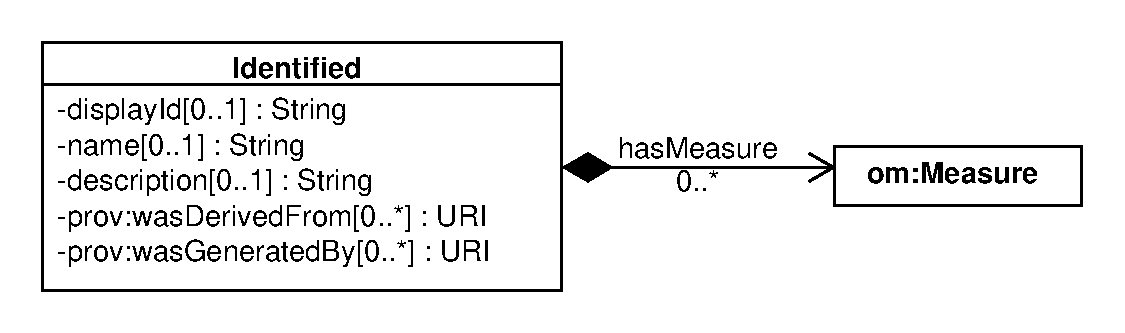
\includegraphics[scale=0.6]{sbol_classes/identified}
\caption[]{Diagram of the \sbol{Identified} abstract class and its associated properties}
\label{uml:identified}
\end{center}
\end{figure}

\begin{itemize}
\item \label{sec:sbol:displayId} 
The \sbol{displayId} property is an OPTIONAL identifier with a data type of \paml{string} (and REQUIRED for objects with URL identifiers). This property is intended to be an intermediate between a URI and the \sbol{name} property that is machine-readable, but more human-readable than the full URI of an object.
If set, its \paml{string} value MUST be composed of only alphanumeric or underscore characters and MUST NOT begin with a digit.

\item \label{sec:sbol:name}
The \sbol{name} property is OPTIONAL and has a data type of \paml{string}. This property is intended to be displayed to a human when visualizing an \sbol{Identified} object.
If an \sbol{Identified} object lacks a name, then software tools SHOULD instead display the object's \sbol{displayId} or URI.

\item \label{sec:sbol:description}
The \sbol{description} property is OPTIONAL and has a data type of \paml{string}. This property is intended to contain a more thorough text description of an \sbol{Identified} object.

\item \label{sec:prov:wasDerivedFrom}
The \prov{wasDerivedFrom} property MAY contain any number of \paml{URI}s. This property is defined by the PROV-O ontology and is located in the \url{https://www.w3.org/ns/prov#} namespace.

\item \label{sec:prov:wasGeneratedBy}
The \prov{wasGeneratedBy} property MAY contain any number of \paml{URI}s. This property is defined by the PROV-O ontology and is located in the \url{https://www.w3.org/ns/prov#} namespace.

\item \label{sec:sbol:hasMeasure}
The \sbol{hasMeasure} property MAY contain any number of \paml{URI}s, each of which refers to a \om{Measure} object that describes a measured parameter for this object.
\end{itemize}

\subsubsection{sbol:TopLevel}
\label{sec:sbol:TopLevel}

\sbol{TopLevel} is an abstract class that is extended by any \sbol{Identified} class that can be found at the top level of a PAML or SBOL document or file.
In other words, \sbol{TopLevel} objects are never nested inside of any other object as a child object.
The \sbol{TopLevel} classes defined in PAML are \paml{Protocol} and \paml{Primitive}. 

\begin{figure}[ht]
\begin{center}
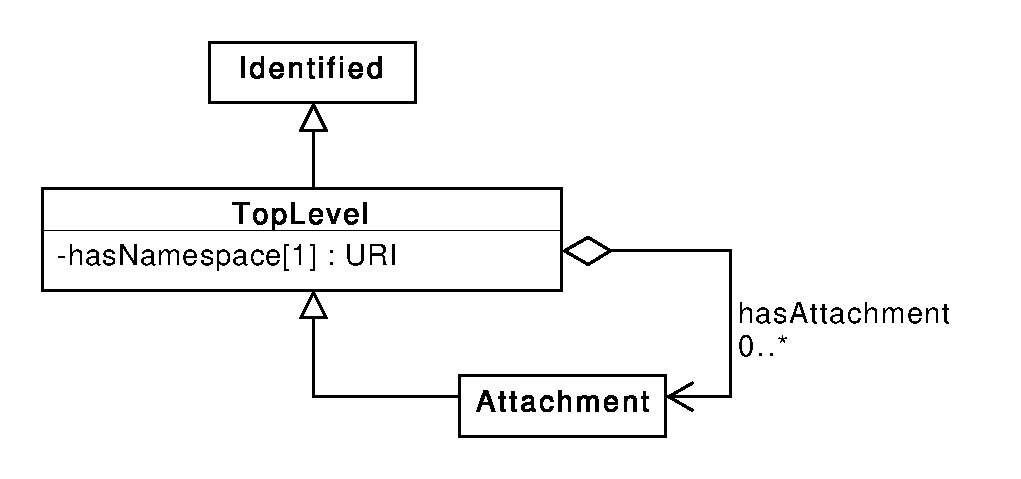
\includegraphics[scale=0.6]{sbol_classes/toplevel}
\caption[]{Classes that inherit from the \sbol{TopLevel} abstract class.}
\label{uml:toplevel}
\end{center}
\end{figure}

\begin{itemize}
\item \label{sec:sbol:hasNamespace}
The \sbol{hasNamespace} property is REQUIRED and MUST contain a single \paml{URI} that defines the namespace portion of URLs for this object and any child objects.
If the URI for the \sbol{TopLevel} object is a URL, then the URI of the \sbol{hasNamespace} property MUST prefix match that URL.

\item 
\label{sec:sbol:hasAttachment}
The \sbol{hasAttachment} property MAY have any number of \paml{URI}s, each referring to an \external{sbol:Attachment} object.
\end{itemize}


\subsubsection{sbol:Component}
\label{sec:sbol:Component}

The \sbol{Component} class represents the structural and/or functional entities of a biological design. 
In PAML, this is primarily used to represent the design of experimental samples as combinations of entities such as strains, genetic constructs, media, inducers, etc.

As shown in \ref{uml:component}, the \sbol{Component} class describes a design entity using a number of different properties.
In many PAML usages, however, a \sbol{Component} will simply be used as a pointer to an external description of a material to be manipulated, and the only property required for interpreting PAML will be \sbolmult{type:C}{type}.

\begin{figure}[ht]
\begin{center}
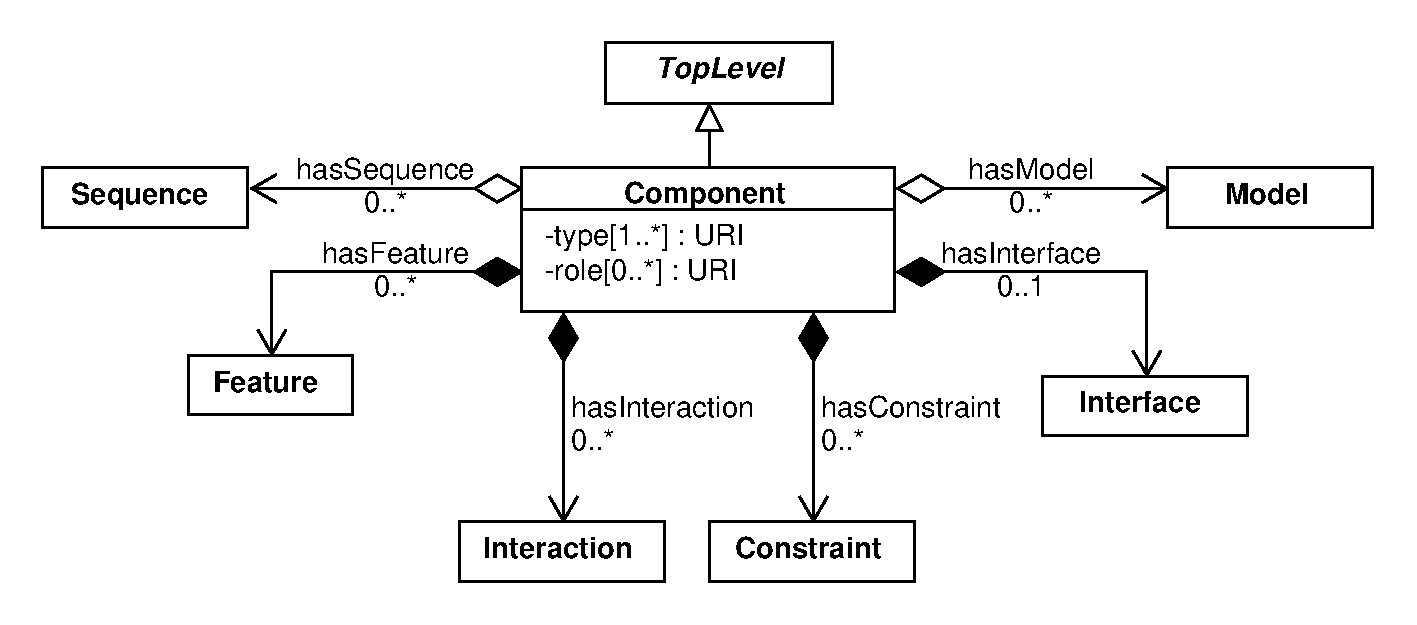
\includegraphics[scale=0.6]{sbol_classes/component}
\caption[]{Diagram of the \sbol{Component} class and its associated properties.}
\label{uml:component}
\end{center}
\end{figure} 

\begin{itemize}
\item \label{sec:sbol:type:C}
The \sbolmult{type:C}{type} property MUST have one or more \paml{URI}s specifying the category of biochemical or physical entity (for example DNA, protein, or simple chemical) that a \sbol{Component} object represents.

\item \label{sec:sbol:hasFeature}
The \sbol{hasFeature} property MAY have any number of \paml{URI}s, each referencing a \sbol{Feature} object. Each \sbol{Feature} represents a specific occurrence of a part, subsystem, or other notable aspect within that design, such as an ingredient in the composition of a growth medium.
\\{\em This is not typically required for specifying protocols in PAML.}

\item \label{sec:sbol:role:C}
The \sbolmult{role:C}{role} property MAY have any number of \paml{URI}s, which MUST identify terms from ontologies that are consistent with the \sbolmult{type:C}{type} property of the \sbol{Component}. 
\\{\em This is not typically required for specifying protocols in PAML.}

\item \label{sec:sbol:hasSequence:C}
The \sbolmult{hasSequence:C}{hasSequence} property MAY have any number of \paml{URI}s, each referencing a \external{sbol:Sequence} object.  These objects define the primary structure or structures of the \sbol{Component}.
\\{\em This is not typically required for specifying protocols in PAML.}

\item \label{sec:sbol:hasConstraint}
The \sbol{hasConstraint} property MAY have any number of \paml{URI}s, each referencing a \external{sbol:Constraint} object.
These objects describe, among other things, any restrictions on the relative, sequence-based positions and/or orientations of the \sbol{Feature} objects contained by the \sbol{Component}, as well as spatial relations such as containment and identity relations.
\\{\em This is not typically required for specifying protocols in PAML.}

\item \label{sec:sbol:hasInteraction}
The \sbol{hasInteraction} property MAY have any number of \paml{URI}s, each referencing an \external{sbol:Interaction} object describing a behavioral relationship between \sbol{Feature}s in the \sbol{Component}.
\\{\em This is not typically required for specifying protocols in PAML.}

\item \label{sec:sbol:hasInterface}
The \sbol{hasInterface} property is OPTIONAL and MAY have a \paml{URI} referencing an \external{sbol:Interface} object that indicates the inputs, outputs, and non-directional points of connection to a \sbol{Component}.
\\{\em This is not typically required for specifying protocols in PAML.}

\item \label{sec:sbol:hasModel}
The \sbol{hasModel} property MAY have any number of \paml{URI}s, each referencing a \external{sbol:Model} object that links the \sbol{Component} to a computational model in any format.
\\{\em This is not typically required for specifying protocols in PAML.}
\end{itemize}

\subsection{TODO: PROV-O imports}
\todo[inline]{Add PROV-O imports here}

\subsection{Ontology of Units of Measure}

In most cases where a number is needed in PAML, that number is a measure with units associated with it.
The Ontology of Units of Measure (OM) (\url{http://www.ontology-of-units-of-measure.org/resource/om-2}) already defines a data model for representing measures and their associated units. 
A subset of OM, already adopted by SBOL, is used for this purpose by PAML as well.

The key class used is \om{Measure}, which associates a number with a unit and a biology-related property.
In most cases, it should be possible to use one of the \external{om:Unit} instances already defined by OM; when this is not possible, an appropriate unit can be defined using \external{om:Unit} and \external{om:Prefix} classes.

\subsubsection{om:Measure} \label{sec:om:Measure}

The purpose of the \om{Measure} class is to link a numerical value to a \external{om:Unit}. 

\begin{itemize}
\item \label{sec:om:hasNumericalValue}
The \om{hasNumericalValue} property is REQUIRED and MUST contain a single \paml{float}.

\item \label{sec:om:hasUnit:Measure}
The \ommult{hasUnit:Measure}{hasUnit} property is REQUIRED and MUST contain a \paml{URI} that refers to a \external{om:Unit}. 

\item \label{sec:sbol:type:Measure}
The \sbolmult{type:Measure}{type} property MAY contain any number of \paml{URI}s. It is RECOMMENDED that one of these \paml{URI}s identify a term from the Systems Description Parameter branch of the Systems Biology Ontology (SBO) (\url{http://www.ebi.ac.uk/sbo/main/}). This \sbolmult{type:Measure}{type} property was added by SBOL to describe different types of parameters 
(for example, rate of reaction is identified by the SBO term \url{http://identifiers.org/SBO:0000612}).
\end{itemize}

\subsection{Recommended Ontologies for External Terms}
\label{sec:recomm_ontologies}

External ontologies and controlled vocabularies are an integral part of SBOL and thus used by PAML as well. SBOL uses \paml{URI}s to access existing biological information through these resources. 
Although RECOMMENDED ontologies have been indicated in relevant sections where possible, other resources providing similar terms can also be used. A summary of these external sources can be found in \ref{tbl:preferred_external_resources}.
The URIs for ontological terms SHOULD come from \url{identifiers.org}.  However, it is acceptable to use terms from \url{purl.org} as an alternative, for example when RDF tooling requires URIs to be represented as compliant QNames, and software may convert between these forms as required.

\begin{table}[htp]
  \begin{edtable}{tabular}{p{2cm}p{1.5cm}p{5cm}p{6cm}}
    \toprule
    \textbf{SBOL Entity} & \textbf{Property} & \textbf{Preferred External Resource}
    & \textbf{More Information} \\
    \midrule
    \textbf{Component}  & type & SBO (physical entity branch)& \url{http://www.ebi.ac.uk/sbo/main/}\\
                                  & type & SO (nucleic acid topology)& \url{http://www.sequenceontology.org}\\
    						   	  & role & SO (\textit{DNA} or \textit{RNA}) & \url{http://www.sequenceontology.org}   \\
    						   	  & role & CHEBI (\textit{small molecule}) & \url{https://www.ebi.ac.uk/chebi/}   \\
							  & role & PubChem (\textit{small molecule}) & \url{https://pubchem.ncbi.nlm.nih.gov/} \\
    						   	  & role & UniProt (\textit{protein}) & \url{https://www.uniprot.org/}  \\   
    						   	  & role & NCIT (\textit{samples}) & \url{https://ncithesaurus.nci.nih.gov/}  \\   
    \textbf{om:Measure}	& type & SBO (systems description parameters) &
    \url{http://www.ebi.ac.uk/sbo/main/} \\
    \bottomrule
  \end{edtable}
  \caption{Preferred external resources from which to draw values for various SBOL properties.}
  \label{tbl:preferred_external_resources}
\end{table}

